\chapter{MC-MP2 Calculations of Dimer Systems}

To demonstrate the efficacy of MC-MP2 method I improved upon, the MC-MP2 method
was applied to a subset of the S22 data set of interacting dimers \cite{s22};
namely the \hho, \ch, \ce{C6H6} (T-shaped), \ce{C6H6} (parallel-displaced)
dimers. Specifically, we wished to determine the \emph{interaction energy} of
the dimer system, calculated using the expression

\begin{equation}
\Delta E = E_\text{dimer} - E_\text{monomer A} - E_\text{monomer B}.
\end{equation}

\noindent The interaction energy can be thought of the stabilizing energy
generated by non-covalent (i.e.\ van der Waals) interactions between the
monomers, excluding energetic contribution resulting from geometric deformation
upon interaction.

For brevity, the benzene dimers will be hereafter be denoted by \benzT,
\benzpara\ respectively. The following chapter details the results of this
investigation.

\section{3D Dimer Geometries}

For the readers' convenience, this section exhibits the 3D geometries of the
dimers chosen for analysis via the MC-MP2 method.

\begin{figure}[H]
\centering
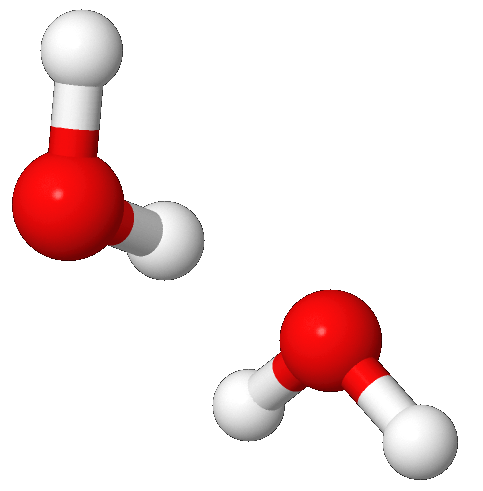
\includegraphics[width = 0.5\textwidth]{figures/h2o.png}
\caption{3D geometry of \hho\ dimer.}
\end{figure}

\begin{figure}[H]
\centering
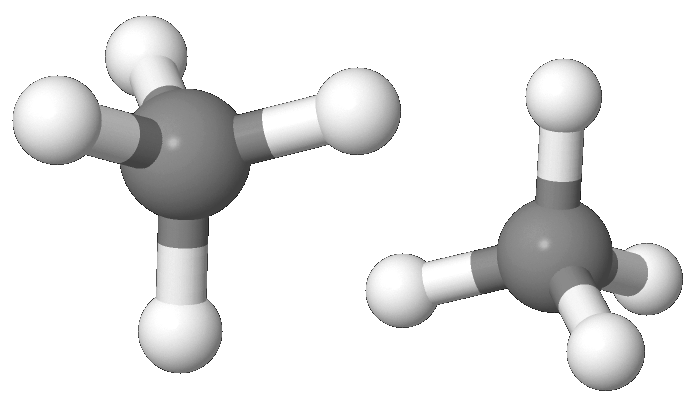
\includegraphics[width = 0.5\textwidth]{figures/ch4.png}
\caption{3D geometry of \ch\ dimer.}
\end{figure}

\begin{figure}[H]
\centering
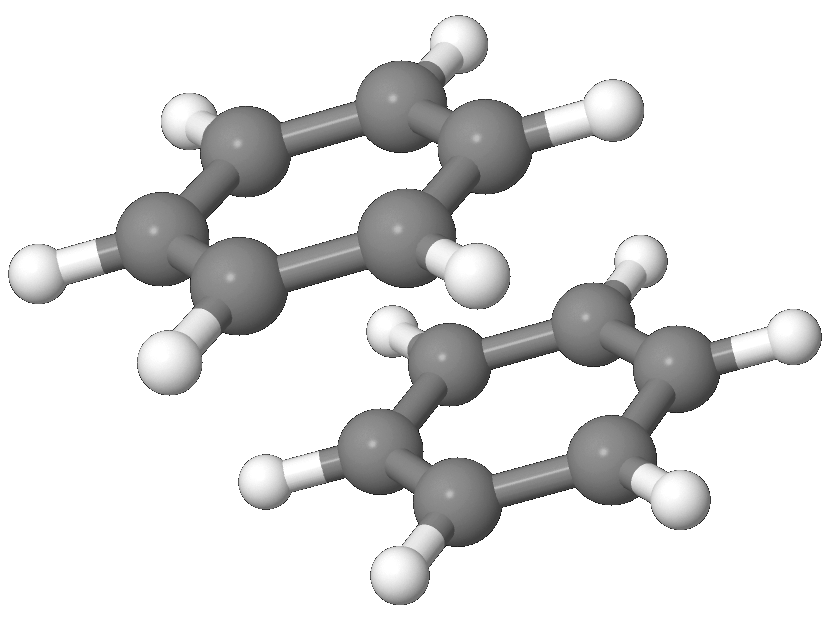
\includegraphics[width = 0.5\textwidth]{figures/benzene-parallel-displaced.png}
\caption{3D geometry of \benzpara\ dimer.}
\end{figure}

\begin{figure}[H]
\centering
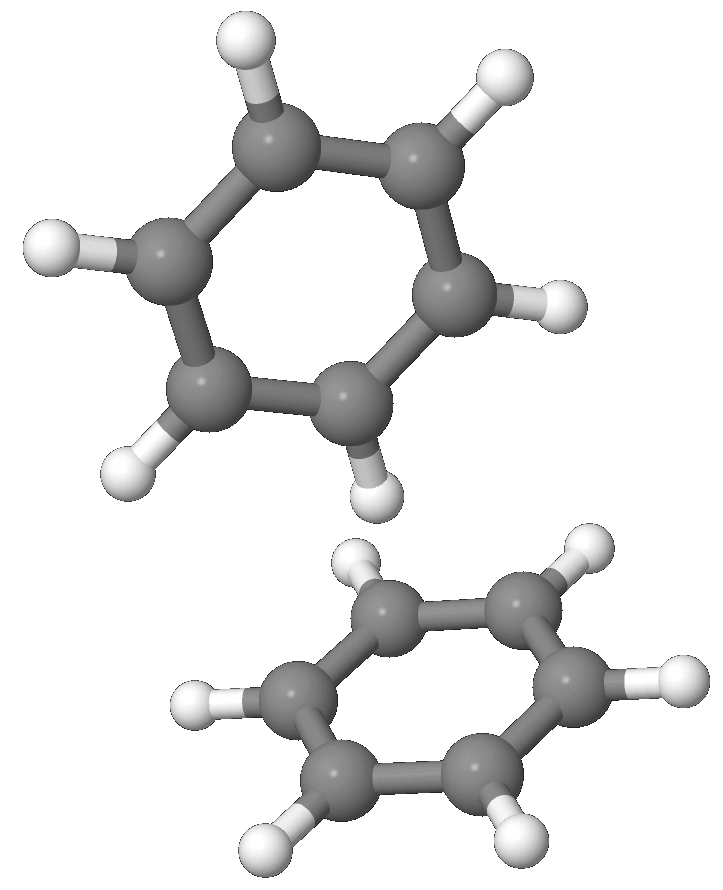
\includegraphics[width = 0.5\textwidth]{figures/benzene-T-shaped.png}
\caption{3D geometry of \benzT\ dimer.}
\end{figure}

\section{HF Interaction Energies}

For each dimer system, the aug-cc-pVDZ basis set \cite{dunning} was used for HF
and MC-MP2 calculations. The SCF method was repeated until the norm of the
orbital gradient was less than $1.0 \times 10^{-8}$ using the NWChem software
suite \cite{nwchem}. CP correction was implemented for the monomer systems by
introducing dummy atoms to NWChem.

\begin{table}[hbt!]
\centering
\caption{Calculated HF interaction energies (kcal/mol) of various molecular dimers.}
\vspace{1em}
\begin{tabular}{ll}
\toprule
Dimer     & $\Delta E_\text{HF}$   \\ \midrule
\hho      & --3.568396             \\
\ch       &  +0.360115             \\
\benzT    &  +1.515152             \\
\benzpara &  +5.353542             \\ \bottomrule
\end{tabular}
\label{t:hf}
\end{table}


As shown in Table \ref{t:hf}, the HF method gives exceedingly poor overestimates
of non-covalent interactions which stabilize dimer systems, thus demonstrating
the necessity of post-HF methods to analyze molecular dimers.

\section{MC-MP2 Computational Details}

This section details how the MC-MP2 methods were implemented for the calculated
data shown in the rest of this chapter. Calculations were performed across
separate nodes of the Gellmann computing cluster in the School of Chemical
Sciences at the University of Illinois and Urbana-Champaign. Each computing node
consisted of two 8-core AMD Opteron 6136 CPUs (2.4 GHz) and 64 GB of RAM.

The MC-MP2 calculations were implemented with full generation of the (6) control
variates. 64 two-electron walkers and 32 one-electron walkers were used by the
redundant walker algorithm. The correlated sampling method was implemented, and
MC-MP2 calculations of the monomers used the random seed of their respective
dimer. The CP-corrected MO basis generated by the preceding HF calculations were
used for the monomers.

\section{MC-MP2 Interaction Energies}

The MC-MP2 and MC-MP2-F12-VBX energies of the selected dimer systems were
calculated. The results are detailed and analyzed in the remainder of this
section.

\begin{table}[hbt!]
\centering

\caption{Calculated MC-MP2 interaction energy correction (kcal/mol) of various
	molecular dimers, with 25,165,824 steps. $\Delta E_\text{MP2}$ and
	$s_\text{MP2}$ represent the estimate of the MP2 energy correction and
	its standard error, respectively. $\Delta E_\text{HF+MP2}$ is the final
	calculated dimer interaction energy obtained with the MC-MP2 method.}

\vspace{1em}
\begin{tabular}{lllllll}
\toprule
Dimer           & Method          & $\Delta E_\text{MP2}$  & $s_\text{MP2}$ & $\Delta E_\text{HF+MP2}$          \\
\midrule
\hho            & MP2             & --0.591806             & 0.117697       & --4.160202                        \\
\hho            & MP2-F12-VBX     & --1.095110             & 0.117979       & --4.663506                        \\
\ch             & MP2             & --0.646745             & 0.170536       & --0.286630                        \\
\ch             & MP2-F12-VBX     & --0.712512             & 0.170538       & --0.352397                        \\
\benzT          & MP2             & --6.047780             & 3.428563       & --4.532628                        \\
\benzT          & MP2-F12-VBX     & --6.438581             & 3.428703       & --4.923429                        \\
\benzpara       & MP2             & --0.885701             & 3.939027       &  +4.467841                        \\
\benzpara       & MP2-F12-VBX     & --1.451004             & 3.939076       &  +3.902538                        \\
\bottomrule
\end{tabular}
\label{t:mp2}
\end{table}


As Table \ref{t:mp2} demonstrates, the energies obtained directly from the
MC-MP2 method, even with the redundant walker algorithm implemented, give poor
estimates of the energies for large systems such as the dimers. For both benzene
dimers, the standard error is comparable to the estimate of the interaction
energy itself. The estimates for the interaction energies of the \hho\ and \ch\
dimers, given that they are smaller systems, are reasonable ($\pm 20\%$) in
comparison with the calculated interaction energies implemented conventional MP2
methods and CCSD(T) methods \cite{s22-ccsdt}.

The \hho\ and \ch\ dimers also demonstrate the significance of the F12-VBX
basis set incompleteness correction, as shifts to lower energies greater in
magnitude than the sum of their respective standard errors.

\section{MC-MP2 Controlled Interaction Energies}

\begin{table}[hbt!]
\centering

\caption{Calculated MC-MP2 interaction energy correction (kcal/mol) of various
	molecular dimers \emph{following variance reduction via the control
	variate method}, with 25,165,824 steps. $\Delta E^C_\text{MP2}$ and
	$s^C_\text{MP2}$ represent the estimate of the controlled MP2 energy
	correction and its standard error, respectively. $\Delta
	E^C_\text{HF+MP2}$ is the final calculated dimer interaction energy obtained
	with the controlled MC-MP2 method.}

\vspace{1em}
\begin{tabular}{lllll}
\toprule
Dimer           & Method          & $\Delta E^C_\text{MP2}$ & $s^C_\text{MP2}$ & $\Delta E^C_\text{HF+MP2}$ \\
\midrule
\hho            & MP2             & --0.807803               & 0.013625         & --4.376199                \\
\hho            & MP2-F12-VBX     & --1.311111               & 0.015875         & --4.879507                \\
\ch             & MP2             & --0.754888               & 0.009349         & --0.394773                \\
\ch             & MP2-F12-VBX     & --0.820656               & 0.009383         & --0.460541                \\
\benzT          & MP2             & --4.610668               & 0.377171         & --3.095516                \\
\benzT          & MP2-F12-VBX     & --5.001499               & 0.378417         & --3.486347                \\
\benzpara       & MP2             & --9.013240               & 0.355480         & --3.659698                \\
\benzpara       & MP2-F12-VBX     & --9.578532               & 0.356047         & --4.224990                \\
\bottomrule
\end{tabular}
\label{t:mp2-c}
\end{table}


Table \ref{t:mp2-c} exhibits the extensive applicability of the control variate
method, and its ability to reduce standard error roughly ten-fold. For each of
the above methods, the standard error is well within 10\% of the eestimate of
the interaction energy. Table \ref{t:mp2-c} furthermore validates the findings
in the previous section regarding the significance of the F12 correction. The
interaction energies, especially those computed with the MP2-F12-VBX method, are
in excellent agreement with the interaction energy computed by the CCSD(T)
method \cite{s22-ccsdt}.

\section{Conclusions}

This chapter thus demonstrated the efficacy of MC-MP2 methods to calculate the
non-covalent interaction energies of dimer systems, with competitive accuracy
compared to the CCSD(T) method, all while being highly parallelizable. MC-MP2
has demonstrated itself as a superior alternative to existing computational
methods regarding solutions of the electronic structure problem for relatively
large systems.
